
\begin{document}
\abstract{Balanced Scorecard y Business model canvas son técnicas de análisis empresarial . Ambas técnicas son útiles para mejorar el desempeño organizacional. Pero sus aplicaciones difieren. Ambos se pueden usar junto con los indicadores clave de rendimiento para monitorear y mejorar el rendimiento de la organización. Vamos a entender tanto la técnica en detalle.}

 Abstract\\
Balanced Scorecard and Business model canvas are business analysis techniques. Both techniques are useful to improve organizational performance. But their applications differ. Both can be used together with the key performance indicators to monitor and improve the performance of the organization. We will understand both the technique and the detail.
\newpage

\section{MODELO DIMENSIONAL}
El modelo multidimensional dentro del entorno de las bases de datos, es una disciplina de diseño que se sustenta en el modelo entidad-relación y en las realidades de la ingeniería de texto y datos numéricos. 
Modela las particularidades de los procesos que  ocurren en una organización, dividiéndolos en mediciones y entorno. La medidas son en su mayoría, medidas numéricas, y se les denomina hechos. Alrededor de estos hechos existe un contexto que describe en qué condiciones y en qué momento se registró este hecho. Aunque el entorno se ve como un todo, existen registros lógicos de diferentes características que describen un hecho, por ejemplo, si el hecho referido, es la venta de un producto en una cadena de tiendas, se podría dividir el entorno que rodea al hecho de la cantidad vendida, en el producto vendido, el cliente que lo compró, la tienda y la fecha en que se realizó la venta. A estas divisiones se le denomina dimensiones y a diferencia de los hechos que son numéricos, estos son fundamentalmente textos descriptivos.
Las medidas, como se  expresó anteriormente, se registran en las tablas de hechos, siendo la llave de esta tabla, la combinación de las múltiples llaves foráneas que hacen referencia   a las
dimensiones que describen la ocurrencia de este hecho, en otras palabras, cada una de las llaves extranjeras en las tablas de hecho se corresponden con la llave primaria de una dimensión.

Esta técnica goza de una gran aceptación y, a menudo, es elegida como la preferida para representar datos analíticos por cumplir simultáneamente con los siguientes requerimientos:\\
Dispone y estructura los datos de manera comprensibles para el usuario de negocio
Genera un alto rendimiento en las búsquedas desde la capa de reporting
Dentro del modelado de datos dimensional destacan 2 conceptos clave: hechos y dimensiones.

Hechos: Son las métricas, normalmente valores cuantitativos (numéricos) susceptibles de ser agregados
Ejemplo: La cantidad de ventas de coches de un concesionario, el rendimiento en euros de una empresa, el número de estudiantes de un colegio, etc.
Dimensiones: Son los valores cualitativos. Proporcionan descripciones a los hechos, aportando un contexto a los mismos.
Ejemplo: Marca de coche, fecha, nombre concesionario, dirección de la empresa, nombre del colegio, etc.
Existen 2 técnicas para llevar acabo el modelado dimensional: el esquema de estrella y el esquema de copo de nieve.
\begin{center}
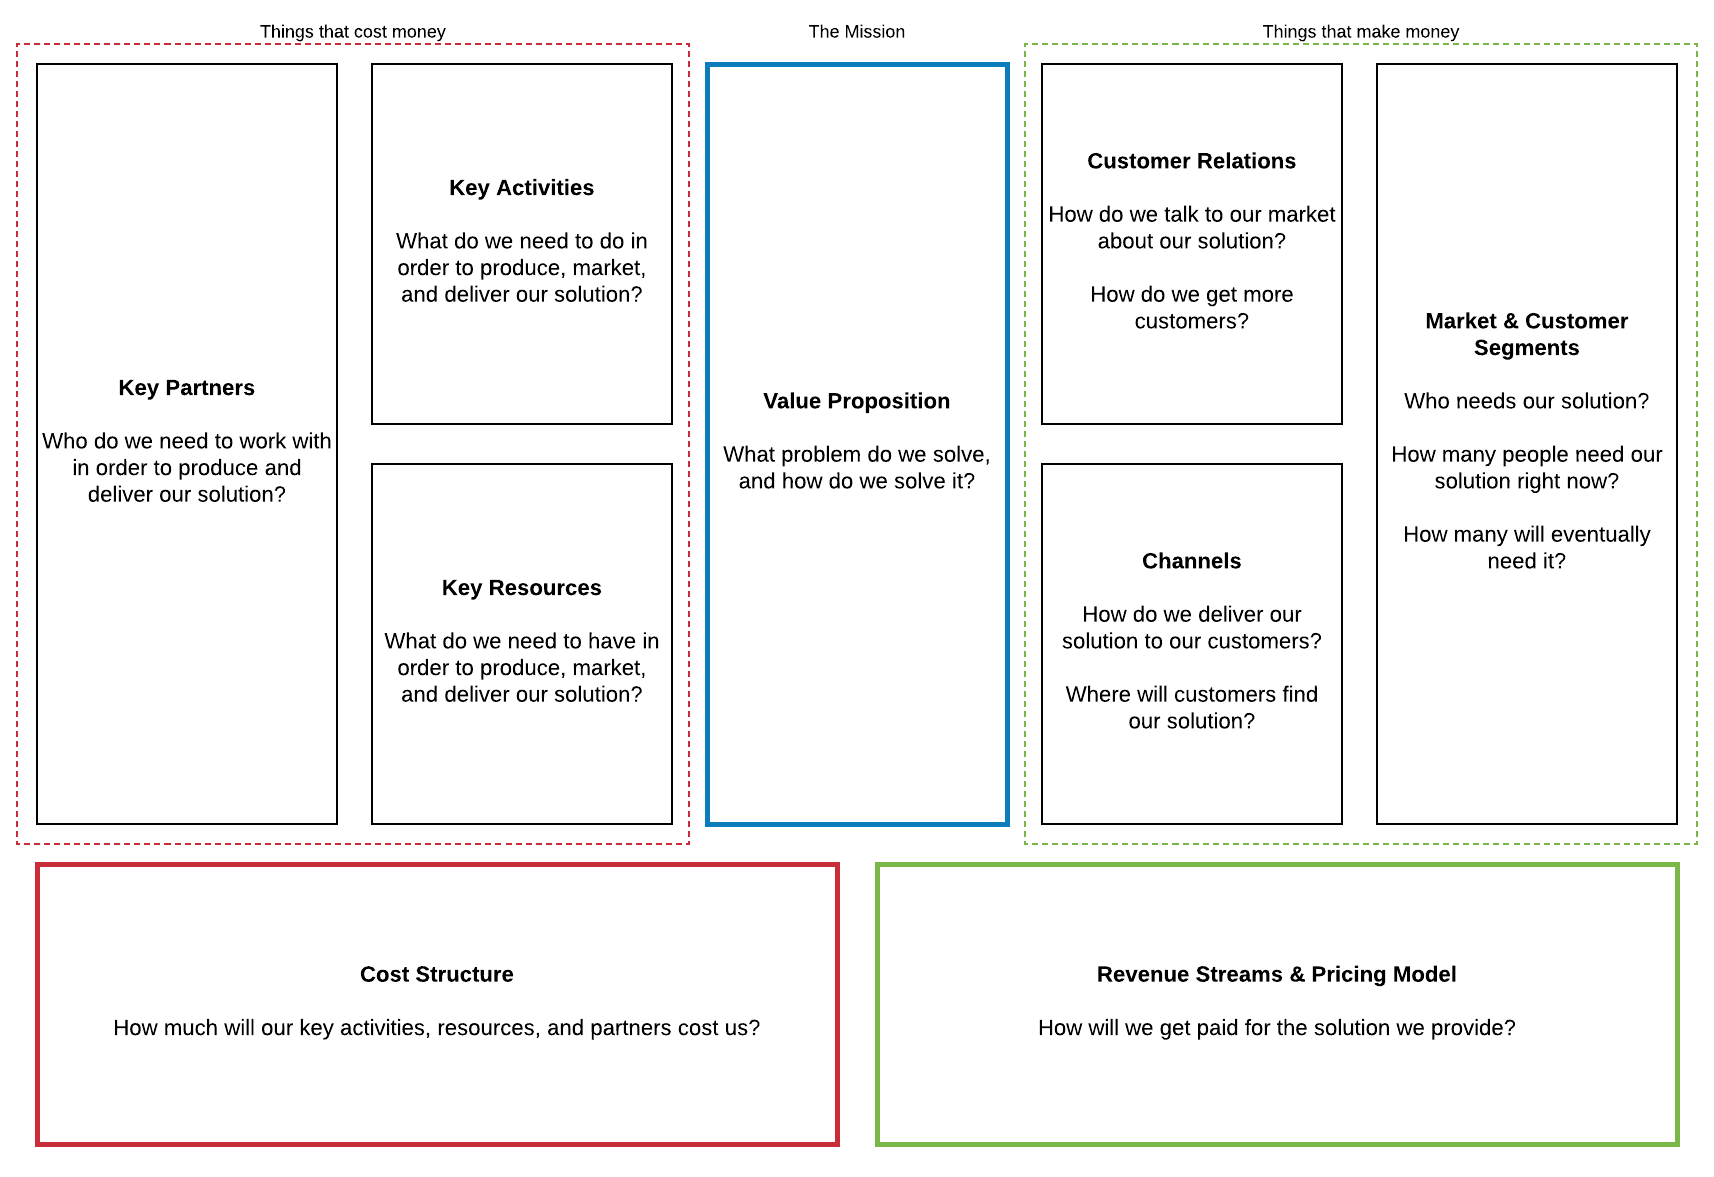
\includegraphics[width=10cm]{./Imagenes/imagen5}
\end{center}


% Bibliografía.
%-----------------------------------------------------------------
\begin{thebibliography}{99}
https://www.isotools.org/2015/02/23/que-es-el-balanced-scorecard-conoce-su-funcionamiento-y-ventajas/\\
https://economipedia.com/definiciones/modelo-canvas.html\\
http://www.infoviews.com.mx/Bitam/ScoreCard/]\\
https://innokabi.com/canvas-de-modelo-de-negocio/\\
https://josefacchin.com/modelo-canvas-de-negocio/\\
https://www.adaptiveus.com/balanced-scorecard-vs-business-model-canvas/\\

\bibitem{Cd94} Autor, \emph{Título}, Revista/Editor, (año)

\end{thebibliography}

\end{document}
